\chapter{Contributions}
\label{cha:contributions}




\section{CycleSense}
\label{sec:cyclesense}
In recent years, more and more cities worldwide aim to reduce the modal share of car traffic in favor of bicycle traffic to reduce NO\textsubscript{x}, CO\textsubscript{2}, and particulate matter emissions, to reduce traffic jams, and to free up space that is urgently needed for other purposes ranging from vegetation that provides natural cooling in a heating world to new flats for a growing population.

A key mechanism to support this is to make bicycle traffic more attractive.
In practice, however, what keeps people from using their bikes more frequently is a lack of safety or perceived safety in cities with a car-centric traffic infrastructure~\cite{aldred2018predictors}.
Hence, city planners urgently require an overview of safety and perceived safety in their city.

Aside from actual accidents, an often overlooked aspect of cycling safety are near miss incidents\footnote{In the remainder of this paper, we will also refer to them as ``incidents''.} such as close passes or near dooring~\cite{aldred2018predictors, karakaya2020simra}.
Information on these have previously not been available or have not been easily accessible as they are distributed over private video recordings, social media posts, public CCTV footage, and other sources.
In 2019, we therefore launched the SimRa\footnote{SimRa is a German acronym for safety in bicycle traffic.} project in which cyclists record their rides and annotate them with incident information via a smartphone app~\cite{karakaya2020simra}.

While our previous approach~\cite{karakaya2020simra} already used a rudimentary heuristic for automatically detecting incidents based on acceleration sensors, it is inherently limited resulting in significant manual annotation efforts which makes it unattractive for some groups of cyclists -- in particular, elderly cyclists who have problems using smartphone apps and cyclists with significant daily mileage for whom the labeling approach is too much effort.
To increase participation, it is hence crucial to decrease manual efforts through an improved pre-detection of incidents.

As a first step towards this goal, we supervised a master's thesis which developed a neural network-based method for incident detection using the public SimRa data set\footnote{https://github.com/simra-project/dataset}~\cite{sanchez2020detecting} which, however, does not show the desired detection quality despite being an improvement over our original heuristic.
Both detection methods are currently used in the live version of the app, hence, we will later use them as baseline in our evaluation.
Besides that, there are alternative approaches for quantifying the perceived safety of bicycle traffic, e.g.,~\cite{blanc2016modeling, blanc2017safety, wu2018predicting}, but to the best of our knowledge no other methods are based on mobile motion sensory data.

Since its start in 2019, the SimRa data set has grown to more than 65,000 rides with almost 30,000 reported incidents.
These amounts of data now enable the application of much more sophisticated methods, namely \ac{ml} and/or \ac{dl}, for automatic incident detection.
Therefore, we here propose CycleSense -- a \ac{dl} model trained on smartphone sensory data from the SimRa data set to detect incidents in the SimRa app.
We hope, that it will lead to more reported incidents due to an easier reporting, and make the following contributions:

\begin{itemize}
	\item We propose an approach that combines signal processing and \ac{ml} techniques to detect incidents based on motion sensor data of cyclists with an \ac{auc} \ac{roc} of 0.906 (Section~\ref{sec:detecting}).
	\item We evaluate our approach using the SimRa data set and compare it to two baselines as well as common \acl{dl} models used in the context of \acl{tsc} (Section~\ref{sec:eval}).
	\item We discuss to which degree our approach can automate incident detection and which additional sensors are needed for full automation (Section~\ref{sec:disc}).
\end{itemize}


\subsection{Detecting Near Miss Incidents}
\label{subsec:detecting_near_miss_incidents}
This section describes the process of automatically detecting incidents. 
Please note that the SimRa data are not optimized for automated processing and \ac{ml} but rather for aggregated statistics and review by humans.
Therefore, several preprocessing steps are needed (Section~\ref{subsec:preprocessing}).
We describe our \ac{ml} model in Section~\ref{subsec:architecture} and the training process in Section~\ref{subsec:training}.


\subsubsection{Preprocessing}
\label{subsubsec:preprocessing}
To overcome some limitations of the SimRa data set, we use data cleaning and preprocessing steps, in a sequential multi-stage manner,  some of which are specific to some model types that will be used afterwards to classify the incidents within rides.

Before the preprocessing phase, a typical ride can be expressed by a $n \times d$ sparse matrix $X^{(i)}$, where $d$ describes the number of sensor features and $n$ represents the number of timestamps in a given ride $i \in \{1,...,R\}$.

Note that we typically only use the accelerometer, gyroscope, and \ac{gps} sensor features.
Using the linear accelerometer features in addition did not lead to a significant improvement.
Furthermore, the linear accelerometer and the rotation vector features are only available in the newer Android rides.
The non-sensory features such as phone location and bike type have a non-logical strong correlation with incidents caused by issues in the data recording phase and are therefore not used.

\begin{figure}[t]
	\centering
	\includegraphics[width=0.5\textwidth]{fig/accelerometer-x-axis.png}
	\caption{The accelerometer readings of an example ride. The encircled spots could indicate an incident but also driving over a curb.}
	\label{fig:x-axis}
\end{figure}

The preprocessing pipeline starts off with a manual label cleaning procedure that aims to remove some of the wrongly labeled incidents.
Identifying them solely based on time series data is practically impossible for a human.
When visualizing the accelerometer sensor readings, incidents usually stand out as sudden spikes (see Figure~\ref{fig:x-axis}), but they also could be caused by driving over a curb or suddenly stopping due to a red light.
Therefore we focus on the incidents that feature an additional description that was provided by the users.
As it is very time-consuming, this is the only manual preprocessing step, and we apply it only to the newer Android data set.
Note that this procedure did not result in a fully cleaned data set.
Next, the timestamps within rides are sorted.
Afterwards, we sort out invalid rides, i.e., rides that contain adjacent timestamps that have been recorded with a gap of more than 6 seconds.
Furthermore, we remove outliers based on the statistical definition of outliers by Tukey et al.~\cite{tukey1977exploratory} that characterizes a data point as an outlier if it fulfills one of the equations $Outlier < q_{25} - k \cdot IQR$ or $Outlier > q_{75} + k \cdot IQR$ where the \ac{iqr} is equal to the difference between the upper and lower quartiles \cite{upton1996understanding, zwillinger1999crc}.
The $k$-values we are utilizing are 1.5 for \ac{gps} outliers regarding the accuracy feature and 3.0 for velocity outliers, as we have seen reasonable results for these values.

In a further step, speed is calculated from the distance between two \ac{gps} coordinates and their respective timestamp.
Moreover, the accelerometer and gyroscope sensor data are interpolated to create equidistance over the whole time series.
This is advisable, as unevenly spaced time series data tend to pose a problem to typical \ac{ml} solutions~\cite{weerakody2021review}.
Therefore, we up-sample to a frequency of 10 Hz via linear interpolation on uniformly generated timestamps with a 100 ms interval.
That means the up-sampling factor is usually above 2.
Although some argue that interpolation is a bad solution for unevenly spaced time series data in the context of \ac{tsc}~\cite{hayashi2005covariance, eckner2012framework}, initial experiments have shown that this improves model performance.
This preprocessing stage results in dense matrices $X^{(i)}$

For better convergence of the stochastic gradient descent optimizer used in the neural network, we normalize each feature individually by its maximum absolute value.
This is nearly always an advantageous preprocessing step as it improves model stability~\cite{bishop1995neural}.

Training the model on individually labeled timestamps did not appear to be a promising approach since incidents have a certain duration, which is typically longer than 100 ms, and it is highly unlikely that the user correctly specifies the label at the exact timestamp when the incident occurred.
For that reason, we split our ride data into 10-second buckets, following a non-overlapping sliding window approach~\cite{ortiz2011dynamic}.
These buckets are then labeled in the following manner: we define a bucket as an incident bucket if any timestamp inside that bucket was labeled as an incident.
Otherwise, we define it as a non-incident bucket.

Additionally, we apply a one-dimensional $f$-point \ac{dft} on each dimension of the accelerometer and the gyroscope sensor data contained in a bucket individually.
This results in a more advanced temporal feature extraction approach that exploits the spectral power changes as time evolves by converting the time series from the time domain to the frequency domain~\cite{chen2021deep}.
%An overview of the process is illustrated in Figure~\ref{fig:fft}

%\begin{figure}[t]
%	\centering
%	\includegraphics[width=\textwidth]{fig/fftDetailed.png}
%	\caption{The process of stacking raw sensor signals into buckets and applying \ac{dft}~\cite{chen2021deep}.}
%	\label{fig:fft}
%\end{figure}

To cope with the heavy label imbalance (e.g., $\approx$ 1 : 170 on rides that have recently been recorded on Android devices) that is present in the data, we use a \ac{gan} with a \ac{cnn} architecture to generate augmented data and thereby lower the imbalance gap by 10\% as this has shown to produce good results in our experiments.
The aforementioned $f$-point \ac{dft} is applied on these synthetic incident buckets as well.

\subsubsection{Model Architecture}
\label{subsubsec:model_architecture}
As our problem setting is similar to the \ac{har} task (see Section~\ref{sec:rw}), we build a customized \ac{ann} inspired by the DeepSense architecture proposed by Yao et al.~\cite{yao2017deepsense}.

In a first step, the network input is split based on the sensor that has produced it into accelerometer, gyroscope and \ac{gps} (i.e., velocity).
Simultaneously, the previously Fourier transformed accelerometer and gyroscope data are separated into their real and imaginary parts.

Then, \ac{sf} is applied, a method that considers each sensor individually in order to extract sensor-specific information~\cite{elmenreich2002sensor}. 
Furthermore, it also enables the application of different individual subnets that are varying in complexity for each sensor input.
Each subnet has three convolutional layers that use 64 kernels, kernel sizes between $(3,3,1)$ and $(3,3,3)$, and a stride size of $1$.
While in the first convolutional layer no padding is used, the second and third convolutional layers apply zero-padding which differs from the original DeepSense framework proposed by Yao et al.~\cite{yao2017deepsense}. 
Another difference is that we use 3D-convolution instead of the 2D- and 1D-convolution that were applied in the original model. 
3D-\acp{cnn} are more suitable for detecting spatiotemporal features compared to 2D-\acp{cnn}~\cite{tran2015learning}. 
The described convolutional layers are complemented by batch normalization layers to reduce internal covariate shifts~\cite{ioffe2015batch}, by \ac{relu} activation, and by Dropout layers for regularization.

Our addition of residual blocks is also a slight modification of the original framework. 
The reasoning behind that change is that, in some cases, deeper models might have difficulties in approximating identity mappings by multiple nonlinear layers~\cite{he2016deep}. 
Residual blocks have been applied with great success to overcome this issue~\cite{he2016deep}.

Next, the outputs of the different subnets are merged in a convolutional fusion network. 
Its architecture is similar to the individual subnets containing six convolutional layers, residual blocks, batch normalization, \ac{relu} activation, and Dropout. 
The full process is shown in Figure~\ref{fig:sfn}.

\begin{figure}[t]
\centering
    \includegraphics[width=0.4\columnwidth]{fig/sensor-and-fusion-networks.png}
    \caption{The model architecture in a nutshell: Using subnetworks for feature extraction of the different sensors (accelerometer, gyroscope, and \ac{gps}) and afterwards a fusion network to combine the features for final incident recognition~\cite{chen2021deep}.}
    \label{fig:sfn}
\end{figure}

The last big component of CycleSense is a \ac{rnn}.
\ac{rnn} architectures such as \ac{lstm}~\cite{hochreiter1997long} or \acp{gru}~\cite{chung2014empirical} are capable of holding information the network has seen before and using it to make predictions in the current state. 
In doing so, it is possible to identify patterns or relationships inside the timestamps of a bucket or between buckets. 
Similar to Yao et al.\ \cite{yao2017deepsense}, we also chose stacked \ac{gru} cells as they efficiently improve the model capacity~\cite{goodfellow2016deep}.

To determine the optimal set of parameters for training CycleSense, we have conducted a grid search on a variety of hyperparameters, some of which are shown in Figure~\ref{fig:hpo}.

In the following, we use \ac{gps}, accelerometer, and gyroscope data as model input if not indicated otherwise.  
Linear accelerometer data was only used in a few experiments as it is not available in our iOS and older Android data sets.
Our implementation of CycleSense is available on GitHub\footnote{https://github.com/simra-project/CycleSense}.

\begin{figure}[t]
	\centering
	\includegraphics[width=\textwidth]{fig/hpo_results.png}
	\caption{Results of the hyperparameter optimization for the four variables $f$ (the window size), the number of \ac{rnn} units used, the \ac{rnn} cell type utilized, and the learning rate from left to right.}
	\label{fig:hpo}
\end{figure}

\subsubsection{Model Training}
\label{subsubsec:model_training}
For model training, the data set was split randomly into a training set (60\%), a validation set (20\%), and a test set (20\%).
Furthermore, the exact same splits are used for each model to improve comparability.
We trained the final model for 60 epochs on an NVIDIA K80 GPU.
We utilized a \ac{bce} loss function that was updated with Adam optimization, a \ac{sgd} method, a learning rate of 0.0001, and early stopping with a patience value of 10 epochs on the \ac{auc} \ac{roc} of the validation set.
It is important to note that we did not use the complete SimRa data set.
Instead, we used only a smaller subset of more recent rides recorded on Android devices since the heterogeneity of the data set across different versions and operating systems (see Section \ref{sec:disc}) did not allow us to train a model properly on the full data set.
In addition, due to limited access to hardware, we focused predominantly on data originating from the Berlin region if not stated otherwise.

As previously described, one notable challenge we were facing was the extreme label imbalance present in the data.
This is due to the fact that incident buckets are far rarer than non-incident buckets.
To cope with that, we trained our model by using a weighted loss function with the class weights of the train data set as weights.
For example, the class weights were 1 and 170 for the rides that have recently been recorded on Android devices.

While the DeepSense model was trained in a standard fashion, we use stacking during the training of CycleSense.
Stacking (or stacked generalization) is an ensemble learning method that combines the predictions of several different models in order to contribute equally to a collective prediction.

However, we are also not interested in equal contributions of the network since that could overvalue models with a poor performance.
We therefore changed the CycleSense model to an integrated stacking model by adopting the idea of stacked generalization~\cite{wolpert1992stacked}, where the fusion network acts as the meta-learner.
Also, we deviate from a pure stacking model.
This is the case, as the meta-learner does not get any classification output of the subnetworks as input aside from the latent features in the last layer of the subnetworks.
Thereby, the weights of the submodel layers that have been pretrained individually are loaded and frozen, so they are not updated during the training of the whole CycleSense model.
This learning procedure further improved our results as shown in Section~\ref{sec:disc}.

\subsection{Evaluation of CycleSense}
\label{subsec:evaluation_cyclesense}
To evaluate CycleSense' training results, we have to put them into context. 
For this purpose, we compare them to the two detection methods currently used in the app as discussed in Section~\ref{sec:background}.
We give an overview of the changes we made to the baseline methods with the goal of a fair comparison in Section~\ref{subsec:baselines}.
We also describe the metrics that we use to compare our model to the baseline methods (Section~\ref{subsec:metrics}) before presenting the results of our evaluation (Section~\ref{subsec:eval-results}).


\subsubsection{Baselines}
\label{subsubsec:baselines}
The first baseline is our original heuristic~\cite{karakaya2020simra} which is based on the underlying assumption that incidents will often result in sudden acceleration spikes, e.g., when braking or swerving to avoid obstacles.
We made some small changes to this heuristic to enable its compatibility with the \ac{auc} \ac{roc} metric, thus, increasing the comparability with our approach.

As a second baseline, we retrained the \ac{fcn} model from the alternative approach~\cite{sanchez2020detecting}.
We used the original preprocessing pipeline (which differs significantly from the here presented one) but used the full data set as introduced in Section~\ref{sec:background}.
We skipped the under-sampling step, disregarded the phone location and the bike type feature for the reasons mentioned in Section~\ref{subsec:preprocessing}, and used a non-overlapping sliding window approach with 10 second windows for better comparability.

The third baseline is DeepSense~\cite{yao2017deepsense}, which we implemented and trained as the authors describe in their work.
For the differences between DeepSense and CycleSense, see sections~\ref{subsec:architecture} and~\ref{subsec:tsc}.

Based on these changes for improved comparability, we retrained the original model.
We use both baselines for comparison as they are, to our knowledge, the only approaches for (semi-)automatically detecting incidents based on sensory time series data.
Furthermore, they have been developed on the SimRa data set, which enables a fair comparison.

\subsubsection{Metrics}
\label{subsubsec:metrics}
Due to the massive label imbalance already mentioned earlier, common metrics such as accuracy, F1-score, and precision are difficult to interpret.
Moreover, in our scenario it is more important to find the true near miss incidents than to classify non-incidents correctly, as False Positives can be more easily corrected by the user of the SimRa app.
For both reasons, a high number of False Positives is more acceptable than a low number of True Positives, which further limits the usefulness of such metrics like precision, F1-score, or \ac{mcc}.
Therefore, we focus on the \ac{auc} of the \ac{roc} metric, which is insensitive to changes in class distribution~\cite{fawcett2006introduction} while also reporting the respective confusion matrices.

\subsubsection{Evaluation Results}
\label{subsubsec:evaluation_results}
In a first step, we compare CycleSense to the two baselines and common model architectures used in the context of \ac{dl} for \ac{tsc}~\cite{ismail2019deep}.
All of these were trained on the Android data set consisting of more recent rides which provides the best results for all approaches.
Figure~\ref{fig:roc-auc-results} and Table~\ref{tab:roc-auc-results} show the differences in performance.

The \ac{fcn} and CycleSense clearly outperform the modified heuristic (0.621 \ac{auc} \ac{roc}).
However, there is still a big performance gap between our model and the \ac{fcn} model.
While the \ac{fcn} model scores 0.847 \ac{auc} \ac{roc}, CycleSense achieves an \ac{auc} \ac{roc} score of 0.906, i.e., there is a chance of $\approx$ 90.6\% that the model can distinguish correctly between a randomly chosen incident and non-incident bucket.
Furthermore, our model performs better than other model architectures that are common for \ac{dl} in \ac{tsc}~\cite{ismail2019deep}: Auto Encoder, \ac{gaf}, \ac{esn}, and the \ac{cnn}-\ac{lstm} model.
With regard to the increasing model complexity, we clearly see diminishing returns.
We can see this in the example of the rather simple \ac{cnn}-\ac{lstm} model which exhibits a relatively close performance to the much more complex CycleSense model with stacking.
The \ac{cnn}-\ac{lstm} model has $\approx$ 90,000 parameters, while the CycleSense model has $\approx$ 1,100,000 parameters.
As a consequence, the time to evaluate the test set of the newer Android data consisting of 795 rides took 4 seconds with the \ac{cnn}-\ac{lstm} model and 56 seconds using CycleSense on the NVIDIA GPU.

\begin{figure}[t]
	\centering
	\includegraphics[width=0.8\textwidth]{fig/roc_auc_results_legend.png}
	\caption{Comparison of the baselines and common model architectures used in the context of \ac{dl} for \ac{tsc}~\cite{ismail2019deep} with the CycleSense model. Note that all of these models have been trained and evaluated on rides contained in the SimRa data set that have been recorded with more recent versions of the SimRa Android app.}
	\label{fig:roc-auc-results}
\end{figure}

\begin{table}
	\centering
	\resizebox{\columnwidth}{!}{%
	\begin{tabular}{cccccccccc}
		\hline
		\centering
		& \textbf{TN} & \textbf{FP} & \textbf{FN} & \textbf{TP} & \textbf{\ac{auc} \ac{roc}} & \textbf{Precision} & \textbf{Recall} & \textbf{F1-Score} & \textbf{MCC} \\
		\hline\hline
		\textbf{CycleSense} & 107934 & 10893 & 104 & 400 & \cellcolor{yellow}0.906 & \cellcolor{yellow}0.035 & 0.794 & \cellcolor{yellow}0.068 & \cellcolor{yellow}0.156 \\
		\hline
		\textbf{CNN-LSTM} & 106427 & 12400 & 127 & 377 & 0.878 & 0.030 & 0.748 & 0.057 & 0.135 \\
		\hline
		\textbf{FCN} & 100932 & 18500 & 98 & 402 & 0.847 & 0.021 & \cellcolor{yellow}0.804 & 0.041 & 0.115 \\
		\hline
		\textbf{DeepSense} & 106192 & 12635 & 153 & 351 & 0.835 & 0.027 & 0.696 & 0.052 &  0.123 \\
		\hline
		\textbf{GAF} & 98782 & 20045 & 150 & 354 & 0.816 & 0.017 & 0.702 & 0.034 & 0.092 \\
		\hline
		\textbf{ESN} & 101670 & 17157 & 138 & 366 & 0.810 & 0.021 & 0.726 & 0.041 & 0.107 \\
		\hline
		\textbf{Auto Encoder} & 58416 & 60411 & 88 & 416 & 0.691 & 0.007 & 0.825 & 0.014 & 0.041 \\
		\hline
	\end{tabular}%
}
\caption{Comparison of the baselines and common model architectures used in the context of \ac{dl} for \ac{tsc}~\cite{ismail2019deep} with the CycleSense model. See the discussion in Section~\ref{subsec:metrics} about the usefulness of various metrics. Note also that all of these models have been trained and evaluated on rides contained in the SimRa data set that have been recorded with more recent versions of the SimRa Android app. For all models the threshold which optimizes Youden's index\cite{youden1950index} were chosen.}
\label{tab:roc-auc-results}
\end{table}

In another experiment, we include the linear accelerometer sensor values in addition to the accelerometer, gyroscope and \ac{gps} data we used so far.
The result for CycleSense is again an \ac{auc} \ac{roc} of 0.906, although the model requires more memory, training and processing time.
Therefore, we leave out the linear accelerometer feature.

So far, we have predominantly focused on newer rides recorded on the Android version of the SimRa app.
As shown in Figure~\ref{fig:traindonone}, the model performs far worse on the other splits of the data set.
Therefore, it was necessary to train an individual model for each part of the data set. 
This yields far better results (Figure~\ref{fig:individually}).

\begin{figure}[t]
	\centering
	\begin{subfigure}[b]{0.475\textwidth}
		\centering
		\includegraphics[width=\textwidth]{fig/rocauctrainedon73.png}
		\caption{\small CycleSense trained only on the newer Android rides and evaluated on all parts of the data set.}
		\label{fig:traindonone}
	\end{subfigure}
	\hfill
	\begin{subfigure}[b]{0.475\textwidth}
		\centering
		\includegraphics[width=\textwidth]{fig/rocauctrainedindividually.png}
		\caption{\small CycleSense trained and evaluated individually on all parts of the data set. \newline}
		\label{fig:individually}
	\end{subfigure}
	\caption{Comparison of CycleSense trained only on the newer Android rides or individual CycleSense models trained for each part of the data set. Note that only the newer Android data set was manually cleaned.}
	\label{fig:comp-trainedonone-individually}
\end{figure}

As the Berlin region has by far recorded the most rides, we have so far used only those for tuning, training, and evaluating our model.
The SimRa app, however, is deployed in many more regions, so our model is clearly required to perform there, too.
For this reason, we have evaluated the Berlin CycleSense model on the newer Android rides coming from Hanover and Nuremberg.

The outcome of this experiment is visualized in Figure~\ref{fig:different-city-trained-on-berlin}.
It clearly shows, that CycleSense does not perform as good as in Berlin.
Since most regions lack training data, it would not be a feasible solution to train models individually per region in the current stage of the SimRa project.
Instead, we retrain CycleSense on a data set that includes all the rides recorded on the newer versions of the Android app within the Berlin, Nuremberg, and Hanover regions.
The results from Figure~\ref{fig:different-city-trained-individually} show that this clearly improves the performance in these additional regions.
At the same time, the performance on the Berlin data set has declined only slightly (0.029 \ac{auc} \ac{roc}) by comparison.
Nevertheless, the \ac{auc} \ac{roc} for Berlin is still the highest and clearly above Nuremberg, which is well ahead of Hanover.

\begin{figure}[t]
	\centering
	\begin{subfigure}[b]{0.475\textwidth}
		\centering
		\includegraphics[width=\textwidth]{fig/city_comp_before.png}
		\caption{\small Performance of CycleSense trained on the new Android data set of rides recorded in Berlin. \newline}
		\label{fig:different-city-trained-on-berlin}
	\end{subfigure}
	\hfill
	\begin{subfigure}[b]{0.475\textwidth}
		\centering
		\includegraphics[width=\textwidth]{fig/city_comp_after.png}
		\caption{\small Performance of CycleSense trained on the new Android data set of rides recorded in Berlin, Nuremberg, and Hanover.}
		\label{fig:different-city-trained-individually}
	\end{subfigure}
	\caption{Comparison of the performance of CycleSense trained on Berlin and trained on the other regions combined.}
\end{figure}

\subsection{Discussion of CycleSense}
\label{subsec:discussion_cyclesense}
Our results demonstrate that the proposed CycleSense model outperforms every other model that we have compared to.
While improving the model's architecture and other components, we identified a number of challenges inherent to the problem setting that we discuss in the following.


\subsubsection{Impact of Preprocessing \& Training Steps}
\label{subsubsec:impact_of_preprocessing_and_training_steps}
In a first step, we want to highlight the importance of our preprocessing and training methods for the success of our model.
Therefore, Figure~\ref{fig:impact} illustrates the performance of CycleSense when one of the preprocessing or training methods is skipped, resulting in a significant drop in performance in each of the four examples.

\begin{figure}[t]
	\centering
	\includegraphics[width=0.5\textwidth]{fig/impact.png}
	\caption{Impact of different preprocessing and training steps on the performance of CycleSense.}
	\label{fig:impact}
\end{figure}

\subsubsection{Limitations of Crowdsourced Data}
\label{subsubsec:limitations_of_crowdsourced_data}
Crowdsourced data are generally noisy which could contribute to a reduced model performance.
They do also contain several biases, e.g., the Selection Bias, Device Positioning Bias, Extreme Aversion Bias, or Confirmation Bias~\cite{basiri2019crowdsourced, chakraborty2017makes, kahneman1991anomalies}.
In this context, the heterogeneity across devices and platforms is likely another factor of influence.
As already described, the application that is used by contributors to record their rides is available on two platforms. 
Those platforms are supported by a wide range of different devices and models with different hardware inside. 
Phone manufacturers use different \ac{gps}, gyroscope, and accelerometer sensors that can vary immensely in sensitivity and overall behavior.
Stisen et al.~\cite{stisen2015smart} have shown that there is major heterogeneity when it comes to the accuracy of sensor readings. 
While the main focus of that study was on accelerometer data, Kuhlmann et al.~\cite{kuhlmann2021smartphone} have shown that orientation sensor data is also affected by this variability.
This is in contrast to the \ac{har} tasks, we compare our task to.
The \ac{har} data set~\cite{anguita2013public} was generated under laboratory conditions that always used the same smartphone type body mounted to the exact same position on selected study participants.
This significantly simplifies the classification task.
Another factor that contributes to the issue of noisy crowdsourcing data in the SimRa data set is the fact that some users misinterpret the purpose of the SimRa app.
Instead of labeling incidents, they report, e.g., dangerous areas or annoying traffic lights.
These can of course not be captured by the sensors used.
Many such ``incidents'' can be identified through the comment column of the data set.
It should also be noted that the SimRa data set was not recorded and labeled with the goal of developing ML models -- the goal was to record data which will be analyzed and processed by humans.

\subsubsection{Technical Limitations of the SimRa Data Set}
\label{subsubsec:technical_limitations_of_the_simra_data_set}
Recording rates of sensor readings deviate among devices and operating systems and impair model predictions~\cite{stisen2015smart}, this may also affect the performance of CycleSense:
As illustrated in Figure~\ref{fig:emp-measurements}, the recording rates differ significantly in older and newer Android rides as well as in iOS rides.
While the iOS rides' median ($\approx$ 300 ms) is similar to the one of newer Android rides, the \ac{iqr} is much greater and spans approximately 150 ms.
This circumstance could indicate that the relatively weak model performance on this data set can partly be explained by that factor. 
Furthermore, the gyroscope data is recorded with a higher frequency in newer Android rides than in older Android or iOS rides.
This factor could also contribute to the different model evaluation results. 
The achieved \ac{auc} \ac{roc} for uncleaned newer Android data was 0.870, while it was 0.823 for the older Android data.

\begin{figure}[t]
	\centering
	\includegraphics[width=0.45\textwidth]{fig/empirical_measurements.png}
	\caption{Box plot showing the empirical measurement times observed in the SimRa data set for rides recorded with different versions of the SimRa app.}
	\label{fig:emp-measurements}
\end{figure}

Aside from that, the moving average that is used in the SimRa app to condense the data and comply to users' upload volume constraints~\cite{karakaya2020simra} reduces the amplitude and shifts the exact point in time of incidents and other events.
This has the effect that incidents and non-incidents are hard to distinguish as illustrated in Figure~\ref{fig:heavy-vs-normal-braking}.
Both these factors could hurt the model's ability to classify incidents correctly based on the data.
It is important to acknowledge that this issue becomes less severe when the sampling frequency is higher, as it is the case for the older Android data.

\begin{figure}[t]
	\centering
	\begin{subfigure}[b]{0.475\textwidth}
		\centering
		\includegraphics[width=\textwidth]{fig/heavy_vs_normal_braking}
		%\caption{\small Scaled accelerometer data over time of the original signal of an artificially modeled incident with heavy braking vs.\ an artificially modeled moderate braking event.}
	\end{subfigure}
	\hfill
	\begin{subfigure}[b]{0.475\textwidth}
		\centering
		\includegraphics[width=\textwidth]{fig/mvn_avg_heavy_vs_normal_braking.png}
		%\caption{\small Moving average applied on the scaled accelerometer data of the original signal of an artificially modeled incident with heavy braking vs.\ an artificially modeled moderate braking event.}
	\end{subfigure}	
	\caption{Visualization of the sensor data of a simulated heavy braking incident vs.\ a moderate braking event before and after the moving average has been applied.}
	\label{fig:heavy-vs-normal-braking}
\end{figure}

\subsubsection{Limitation of the Classification Task}
\label{subsubsec:limitation_of_the_classification_task}
There is an inherent label imbalance present in our data set.
Only relatively few rides contain incidents. 
Moreover, the ratio between timestamps that represent an incident and those that do not is even smaller. 
As a consequence, there is an enormous imbalance between the different label categories.

Furthermore, some incident types such as tailgating or close passes might not be detectable at all in accelerometer and gyroscope sensors~\cite{aldred2018predictors, karakaya2020simra} as cyclists might not change their motion profile despite (or even due to) a dangerous situation.
For detecting these kinds of incidents it may be necessary to include different sensors.
In the SimRa project, this is already happening through an integration of \ac{obs}\footnote{https://www.openbikesensor.org/} data which measures the passing distance of cars.
The current data set, however, only includes very few OBS-supported rides.

In contrast to our classification task, the inherent classification problem of the \ac{har} data set \cite{anguita2013public}, is to classify reoccurring ongoing patterns such as walking or jogging, while an incident might need to be detected by one short non-reoccurring event such as sudden braking.
This further complicates the matter.

\subsubsection{Data Set Shift}
\label{subsubsec:data_set_shift}
A major challenge in the context of crowdsourced data are data set shifts. Depending on the device (see also \autoref{subsec:technical_limitations}), but also on other factors, such as the city of origin of the recorded data (see also \autoref{subsec:eval-results}), there could be non-stationarities in the data that violate the assumptions underlying almost all ML models and thus could impact the generalization performance of the trained models. Several types of data set shifts can be distinguished, including \textit{covariate shifts}, meaning shifts in the input data \cite{sugiyama_machine_2012}, \textit{label shifts}, meaning shifts in the distribution of targets \cite{lipton_detecting_2018}, or mixtures thereof. Detecting these shifts \cite{polyzotis_data_2018, rabanser_failing_2018, breck_data_2019, abdar_review_2021, bates_testing_2021} and predicting \cite{schelter_learning_2020} or reducing their impact on the generalization performance is an active field of research \cite{schelter_challenges_2018, biessmann_automated_2021}. Some approaches aim at model specific improvements to alleviate data set shift \cite{sugiyama_machine_2012}. These approaches have a decisive disadvantage, most of these approaches only work for one model class and require access to the inner workings of the ML pipeline, often after the feature extraction step. More promising and easier to build and maintain are model agnostic solutions that focus on the data, rather than the models, to detect and counteract data set shifts \cite{biessmann_automated_2021}. Extending the training data sets to account for all variation and shifts in the data that the ML model should be invariant to, often called \textit{augmentation}, is a popular and effective way of counteracting data set shift, see for instance \cite{cubuk_autoaugment_2019}. In our work we follow this line of thought of a data centric AI approach. 

\subsection{Summary of CycleSense}
\label{subsec:summary_cyclesense}
An increased modal share of bicycles is necessary for solving emission and traffic related urban problems.
A key challenge for this, is the lack of (perceived) safety for cyclists.
Improving the situation requires detailed insights into safety levels of street segments -- the SimRa platform~\cite{karakaya2020simra} has been proposed as a data gathering mechanism for incidents and cycling tracks.
While this is an important step towards data collection, the platform relies on manual annotation of tracks which limits the number of potential users.

In this paper, we have proposed CycleSense -- a model for automatic detection of such incidents.
Using the SimRa data set, we have shown that CycleSense is capable of detecting incidents on the basis of accelerometer and gyroscope time series data in a real-world scenario.
It can correctly distinguish between an incident and a non-incident with a probability of up to 90.5\%.
We have also compared it to the heuristic currently used in the SimRa platform and an existing \ac{fcn} that was specifically developed for SimRa.
Additionally, we have implemented several \ac{dl} models that are frequently used in the context of \ac{tsc}.
We were able to show that our model outperforms all of these approaches.

While this is an important step towards fully automatic incident detection, we believe that -- in the context of the SimRa platform -- CycleSense should be complemented with human annotation in a semi-automated way for the foreseeable future.
Although this does not quite reach our long-term goal of full automation, it should significantly decrease the annotation effort and should also lead to improved labeling quality.
In the future, this could, in turn, be used to further improve CycleSense.
Since April 2022, the SimRa app has been using CycleSense for incident detection.



\section{CycleQuality}
\label{sec:cyclequality}


Cities all over the world aim to increase the modal share of bicycle traffic, e.g., to address emission problems, frequent traffic jams, but also to improve the citizens' health through more daily activity.
Key factors for this are traffic safety, topography but also the comfort level of cyclists~\cite{Nyberg1996Road,gadsby2022understanding,karakaya2020simra}.
All these factors are affected by the availability and quality of cycling infrastructure which needs to be monitored and maintained continuously.
Even monitoring of surface quality alone, however, can be challenging due to the sheer dimensions of existing infrastructure.
Germany's capital Berlin, for example, has around 2,300 km of bicycle tracks as of March 2023, i.e., manually inspecting cycling infrastructure to monitor surface quality is infeasible.

To address this problem, we propose to use a crowdsensing approach in which cyclists record their daily rides using a smartphone app.
Using the built-in motion sensors, the surface quality (or rather the lack of) can be measured as vibrations or bumps.
In a second step, we can then combine data from multiple rides to derive an estimate for the surface quality.
This way, monitoring of surface quality can be automated to a high degree at little cost and the resulting data can be used for maintenance planning or surface quality-aware routing.
Especially for highly frequented cycling tracks, surface quality problems can be detected quickly.

While there are other projects studying the surface quality of cycling infrastructure through crowdsourcing (e.g., Luedemann et al.~\cite{luedemann2022bikevibes}), our work is unique and novel because alternative approaches (i) either focus on categorizing the surface \emph{type} (e.g., cobblestones) where we focus on the surface \emph{quality} (i.e., the level of roughness) or (ii) have strict assumptions on phone positioning and other properties where we rely on a ``wisdom of the crowds'' strategy to filter out noise.
The latter is also an advantage because, unlike related approaches, which use a dedicated app for measuring the road surface quality, thus, potentially forcing cyclists to run multiple apps, our approach can easily be retrofitted to existing apps and can even be used to analyze already stored datasets.

For this, we make the following contributions:
\begin{itemize}
	\item We present a data processing pipeline for deriving surface quality which combines signal processing with geographical clustering techniques in the form of edge-based preprocessing on the phone and cloud analytics (\cref{sec:pipeline}).
	\item We describe how we integrate this data processing pipeline in the existing crowdsensing project SimRa~\cite{karakaya2020simra} which up to now has only focused on traffic safety(\cref{sec:pipeline}).
	\item We describe how the resulting data can be used to increase the comfort of cyclists through surface quality-aware routing and how the data can be exposed to city administrations(\cref{sec:use}).
	\item We evaluate our approach by analyzing the SimRa dataset~\cite{dataset_simra_set1,dataset_simra_set2,dataset_simra_set3} and comparing it on-site conditions in eight streets with different surface quality (\cref{sec:eval}).
	\item We discuss to which degree our approach can automate surface quality monitoring and how additional sensors could possibly help to improve data quality (\cref{sec:disc}).
\end{itemize}


\subsection{Data Processing Pipeline}
\label{subsec:data_processing_pipeline}
In this section, we start by giving a high-level overview of our data processing pipeline for deriving surface quality \cref{sec:overview} before describing the individual steps in the process (\cref{sec:data_acq} to \cref{sec:surface_quality}).


\subsubsection{Overview of Pipeline}
\label{subsubsec:overview_of_pipeline}
\begin{figure}
    \centering
    \includegraphics[width=\columnwidth]{fig/overview.pdf}
    \caption{%
        Overview of our surface quality analysis pipeline.
    }%
    \label{fig:overview}
\end{figure}
The tasks of our data processing pipelines are distributed over the edge (i.e., on the smartphone) and the cloud, see also \Cref{fig:overview}.
After collecting data in the SimRa app using the built-in motion sensors, data is preprocessed locally before upload to our backend servers.
There, additional preprocessing steps are executed before the actual surface quality analysis.

The parts of the preprocessing which reduce the amount of data need to be run on the edge to preserve user privacy and to reduce bandwidth consumption.
The data cleaning parts are too compute-intensive and are executed in the cloud to reduce power consumption on the phone.

\subsubsection{Preprocessing in the Cloud}
\label{subsubsec:preprocessing_in_the_cloud}
The preprocessing in the cloud has two main goals: cleaning noisy data and calculating a value that represents the smoothness of the ride.
For the first goal, we cut off ten seconds each at the start and end of the ride to remove noise resulting from users (un)mounting their bikes or putting the phone in a pocket.
Ideally, this would of course already be done on the phone but could not be done here since the main use case of SimRa requires this data, i.e., we would have had to upload the data twice.
We also remove stops, i.e., only the parts of the ride which have a minimum speed of 5 km/h and a minimum duration of 1 minute are considered.
Such low speeds usually occur, when the bicycle is being pushed by the cyclist rather than being ridden or when stopping at traffic lights.
Even if the cyclist should manage to ride so slowly, the ride will be prone to unsteady motions, leading to noisy data.
This also removes parts where users forgot to stop the recording after their ride.

For the second goal, we normalize the accelerometer data by calculating the mean of the three moving variances (window size 10) of the axes X, Y and Z.
This preserves information about amplitude but disregards the direction which is highly affected by the position of the phone.
Thus, we obtain a time series of single values representing the bumpiness of the surface in each in-motion ride segment.

\subsubsection{Surface Quality Analysis}
\label{subsubsec:surface_quality_analysis}
Each cyclist creates a different data track on a given road, and without calibration, it is not possible to accurately analyze each track individually.
Ideally, we would at least use cyclist-specific profiles (i.e., per cyclist aggregates) which, however, are not available due to privacy reasons (rides are pseudonymized individually~\cite{karakaya2020simra}).
The idea behind our approach is to take advantage of the size of the data set and use the law of large numbers to obtain robust results without having to calibrate the data and without affecting the results too much by noise.

For this, we consider in the first step each ride individually:
We take the preprocessed ride (which is a single time series of aggregated motion sensor readings without stops plus the GPS trace) and calculate the percentiles (0.2, 0.4, 0.6, 0.8, and 1) of the time series.
For normalization, we then replace all motion sensor readings with values 1 to 5 depending on which interval they fall into, i.e., a motion sensor reading from the interval $(0.2;0.4]$ would be replaced with the value 2.
The intuition behind this is that longer rides are likely to encounter very different surface quality, hence we calculate the relative bumpiness of an area in comparison to the rest of the ride's bumpiness.

In the second step, we use the data from all such normalized rides and, using the GPS trace, map them to a grid of 10m² cells.
For each cell, we hence have a distribution of values 1 to 5.
As a metric for the bumpiness of that cell, we use the average of all values -- e.g., when color-coding a map -- but make other statistical metrics available as well (see, e.g., the distribution function charts in our evaluation section).

\subsection{Using Road Surface Quality Information}
\label{subsec:using_road_surface_quality_information}
In this section, we describe how such surface quality results can be used.
In \cref{sec:routing}, we describe how we implement a navigation feature into the SimRa app that uses the road surface quality as an additional parameter in routing.
We then show in \cref{sec:visualization} how we can expose the output data of our pipeline to city administrators.


\subsubsection{Routing with Surface Quality}
\label{subsubsec:routing_with_surface_quality}
With the surface quality scores calculated, it is possible to provide a route planning feature, where not only distance and time are considered, but also the surface quality.
The main question here is how much the surface quality should be weighed when calculating the best route from A to B or rather what detour lengths are acceptable.
We decided to give the user the opportunity to influence this factor with the usage of a slider, that can be set between 0 for not considering surface quality in the routing and 10 for the highest importance of the surface quality (\cref{fig:routing}).
 \begin{figure}
    \centering
    \includegraphics[width=\columnwidth]{fig/routing_settings_2.png}
    \caption{%
With a slider in the settings menu, the weight of the surface quality in the routing can be set.}%
    \label{fig:routing}
\end{figure}
We host a modified GraphHopper\footnote{https://github.com/graphhopper/} for routing.
GraphHopper uses edges for streets, that are connected via nodes.
Each has a weight for routing purposes and it is possible to change the weight according to custom data.
This is where we use the surface quality by increasing the weight depending on surface quality and user-specified influence factor.

\subsubsection{Output Data and Visualization}
\label{subsubsec:output_data_and_visualization}
Our bicycle road surface quality pipeline creates a GeoJSON file as an output.
It contains the cells with a surface area of 10m² in a grid as \codeword{Features} of the \codeword{geometry} type \codeword{Polygon} with the surface quality score information such as mean, median, standard deviation, number of rides going through the cell and coloring information in the \codeword{properties} key.
 \begin{figure}
    \centering
    \includegraphics[width=\columnwidth]{fig/visualization.png}
    \caption{%
A visualization of the output file showing the surface quality of the boxes when hovering over them with the mouse cursor. Color coding is based on the average value.}%
    \label{fig:visualization}
\end{figure}
With such an output file, it is very easy to create a simple visualization\footnote{https://simra-project.github.io/surfaceQuality/Berlin.html}, e.g., with Leaflet\footnote{https://leafletjs.com/}, as depicted in \cref{fig:visualization}.
Using a visualization like this, also non-tech-savvy users can easily monitor the bicycle road surface quality of a large area and take action where needed.


\subsection{Evaluation of CycleQuality}
\label{subsec:evaluation_cyclequality}
In this section, we evaluate the surface quality analysis by comparing the calculated surface quality of selected street segments across Berlin with their surface type in the real world, which we get from OpenStreetMap (OSM).
As data input, we use the existing SimRa datasets~\cite{dataset_simra_set1,dataset_simra_set2,dataset_simra_set3} (almost 90,000 rides with more than 650,000km in total).
Based on the intuition that different surface types will also be partially correlated with surface quality, we randomly picked four spots with different surface types.
To also show the limitations of our approach, we then explored the dataset and manually picked four additional spots where our approach appears to have returned the wrong results.
Each evaluated section has a surface area of 10 m² and to compare them to each other we analyze their mean, median, and standard deviation values.

We first describe the clear results from the first group (\cref{subsec:clear}).
Afterwards, we categorize the additional four ``problem spots'' as mixed results (\cref{subsec:mixed}) or seemingly incorrect results (\cref{subsec:mismatch}).


\subsubsection{Sections with Clear Results}
\label{subsubsec:sections_with_clear_results}
We evaluate at least one example for each of the following surface types, which are sorted in descending order with regard to their expected surface quality~\cite{titov2019monitoring}: asphalt, flat paving stones, fine gravel, cobblestones.
We chose the sections in a way that (i) asserted that we have sufficient data for them and (ii) to cover all different surface types.
After filtering based on these criteria, we randomly picked four sections.

\cref{tab:clear} and \cref{fig:clear} show the results of the surface quality analysis of the selected sections with very clear and intuitive results.

\begin{figure}
    \centering
    \includegraphics[width=\columnwidth]{fig/pdf_clear.png}
    \caption{%
        The Probability Density Function of the Derived Surface Qualities shows that these segments have very undisputed road surface quality values, since they are either very good or very bad.
    }%
    \label{fig:clear}
\end{figure}

It can be observed, that the aforementioned list of surface types, which was sorted in descending surface quality order, was ordered correctly.
A newly maintained asphalt section in \textit{Straße des 17. Juni} has a nearly perfect score, which means that its surface quality was in the top 20\% in almost all rides crossing this section.
Followed by that are two sections with flat paving stones and fine gravel as their surface type, which have very similar results.
This means, that both flat paving stones and fine gravel have comparable surface quality in terms of bumpiness from the perspective of a cyclist.
However, it should be noted, that fine gravel can be less favorable in areas with a lot of precipitation (more on that in \cref{sec:disc}).
Not very surprisingly, the \textit{Liebauer Straße} has very bad surface quality scores, since it is paved with cobblestones and has very busy sidewalks with restaurants and cafes, which prevent cyclists from (illegaly) cycling there instead of on the street.

\begin{table}%
\centering
\caption{Surface Quality Analysis Evaluation Results Showing Mean, Median and Standard Deviation of Sections With Clear Results}%
\label{tab:clear}
\resizebox{\columnwidth}{!}{
\begin{tabular}{cccccc}%
\toprule%
Street Name          & Surface       & GPS Location        & Mean & Median & Std. Dev.\\%
\midrule%
\midrule%
Straße des 17. Juni  & Asphalt       & 52.515369,13.630855 & 1.03 & 1      & 0.17\\%
Straße des 17. Juni  & Paving Stones & 52.513501,13.335127 & 1.25 & 1      & 0.5\\%
Tiergarten           & Fine Gravel   & 52.514745,13.34622 & 1.32 & 1      & 1.06\\%
Liebauer Straße      & Cobblestones  & 52.509132,13.453806 & 4.15 & 4      & 1.07\\%
\bottomrule&%
\end{tabular}%
}
\end{table}

\subsubsection{Sections with Mixed Results}
\label{subsubsec:sections_with_mixed_results}
While most results are intuitive, e.g., new bicycle roads paved with asphalt and separated from the motorized vehicle traffic having very good surface conditions, some other sections (see \cref{fig:mixed}) seem confusing at the first glance.

\begin{figure}
    \centering
    \includegraphics[width=\columnwidth]{fig/pdf_mixed.png}
    \caption{%
        The Probability Density Function of the Derived Surface Qualities shows that these segments have confusing road surface quality values: Depending on the ride, they appear to have either very good or very bad surface quality (multiple peaks).
    }%
    \label{fig:mixed}
\end{figure}

According to the Probability Density Functions (PDFs) of street sections in the \textit{Invalidenstraße} and \textit{Kaiserin-Augusta-Allee}, there seem to be two distinct surface qualities in each section.
A closer look into the specific sections reveal the causes:
 
\begin{table}%
\centering
\caption{Surface Quality Analysis Evaluation Results Showing Mean, Median and Standard Deviation of Sections With Mixed Results}%
\label{tab:mixed}
\resizebox{\columnwidth}{!}{
\begin{tabular}{cccccc}%
\toprule%
Street Name          & Surface       & GPS Location        & Mean & Median & Std. Dev.\\%
\midrule%
\midrule%
Invalidenstraße           & Asphalt   & 52.526236,13.369196 & 2.24 & 3      & 0.96\\%
Kaiserin-Augusta-Allee      & Asphalt  & 52.524429,13.327253 & 2.17 & 2      & 1.05\\%
\bottomrule&%
\end{tabular}%
}
\end{table}

In \textit{Invalidenstraße}, there are a bus lane, a bus stop, and an on-curb bike lane (see \cref{fig:invaliden}).
Most bus lanes in Berlin can be legally used by cyclists, however, some cyclist may still prefer the relatively bumpy bike lane.
\begin{figure}
    \centering
    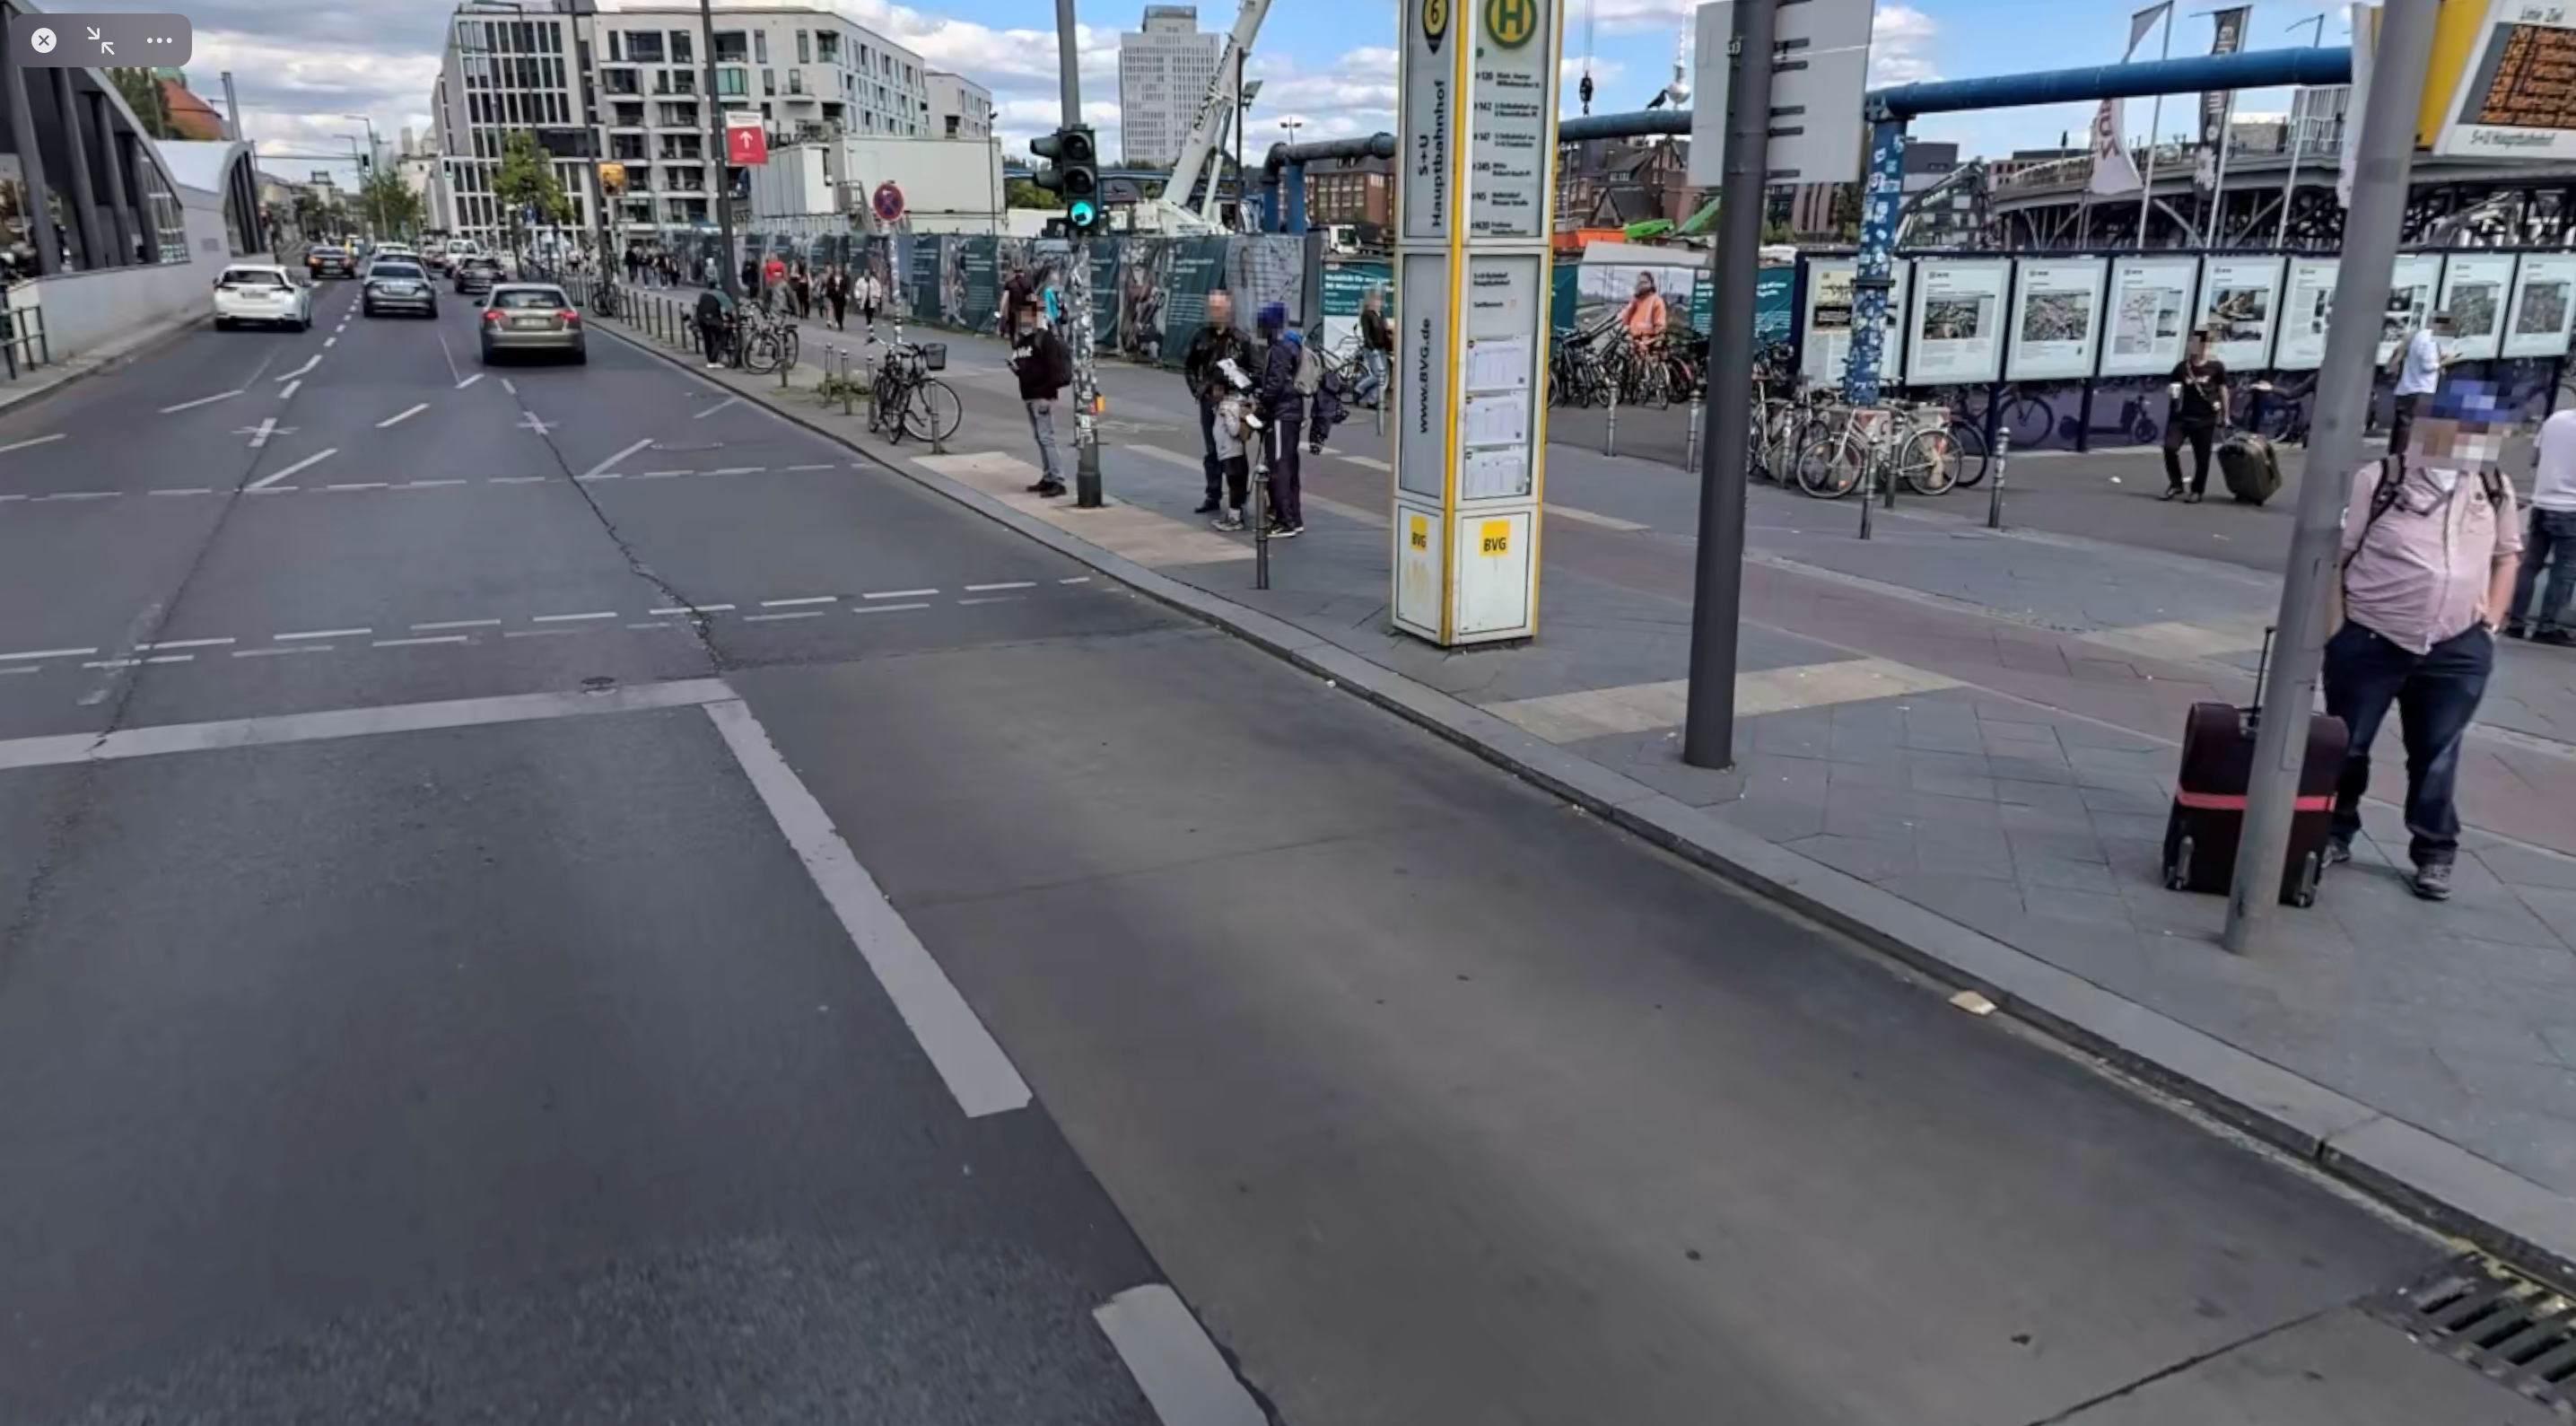
\includegraphics[width=\columnwidth]{fig/invalidenstr.png}
    \caption{%
        A bus lane, a bus station and a bicycle lane on the sidewalk can create different results in a small area. (Source: Apple Maps)
    }%
    \label{fig:invaliden}
\end{figure}
Additionally, when a bus stops at the bus station, cyclists that used the bus lane might overtake the bus on the very smooth car lane to the left. 
These two factors most certainly are the reason for the distinct two-peak distribution of recordings in that spot.

A closer look at the near-miss incident data in \textit{Kaiserin-Augusta-Allee} indicates that people use the bike lane in one direction and the street in the other direction~\cite{dataset_simra_set1,dataset_simra_set2,dataset_simra_set3} as one side seems to be in an unusable condition while the other is acceptable.
Since the bicycle lane is paved with paving stones and the street with asphalt, this leads to different surface quality of the road, depending on which direction the ride was.
Both directions, however, regularly end up in the same 10x10m box as the street is not overly wide, especially considering GPS accuracy.

\subsubsection{Sections with (Seemingly) Confusing Results}
\label{subsubsec:sections_with_seemingly_confusing_results}
There are also sections where the surface quality result seem to be completely wrong, when compared to the OSM surface type labels.
\Cref{tab:mismatch} shows two sections, that are -- according to OSM -- paved with cobblestones and without separate bike lanes, but with very good results, which is confirmed by the PDFs depicted in \cref{fig:mismatched}.

\begin{figure}
    \centering
    \includegraphics[width=\columnwidth]{fig/pdf_mismatched.png}
    \caption{%
        The Probability Density Function of the Derived Surface Qualities shows that these segments have very smooth road surfaces, although they are paved with cobblestones.
    }%
    \label{fig:mismatched}
\end{figure}

The possibility, that this section has a wrong label and is in fact, not paved with cobblestones may come to mind.
However, as \cref{fig:sidewalk} reveals, both streets are indeed paved with cobblestones.

\begin{figure*}[t]
    %\vspace{-3em}
    \centering
    \subfloat[Straßburger Straße]{\includegraphics[width=\columnwidth]{fig/straßburger_str_2.png}}
    \hfill
    \subfloat[Goethestraße]{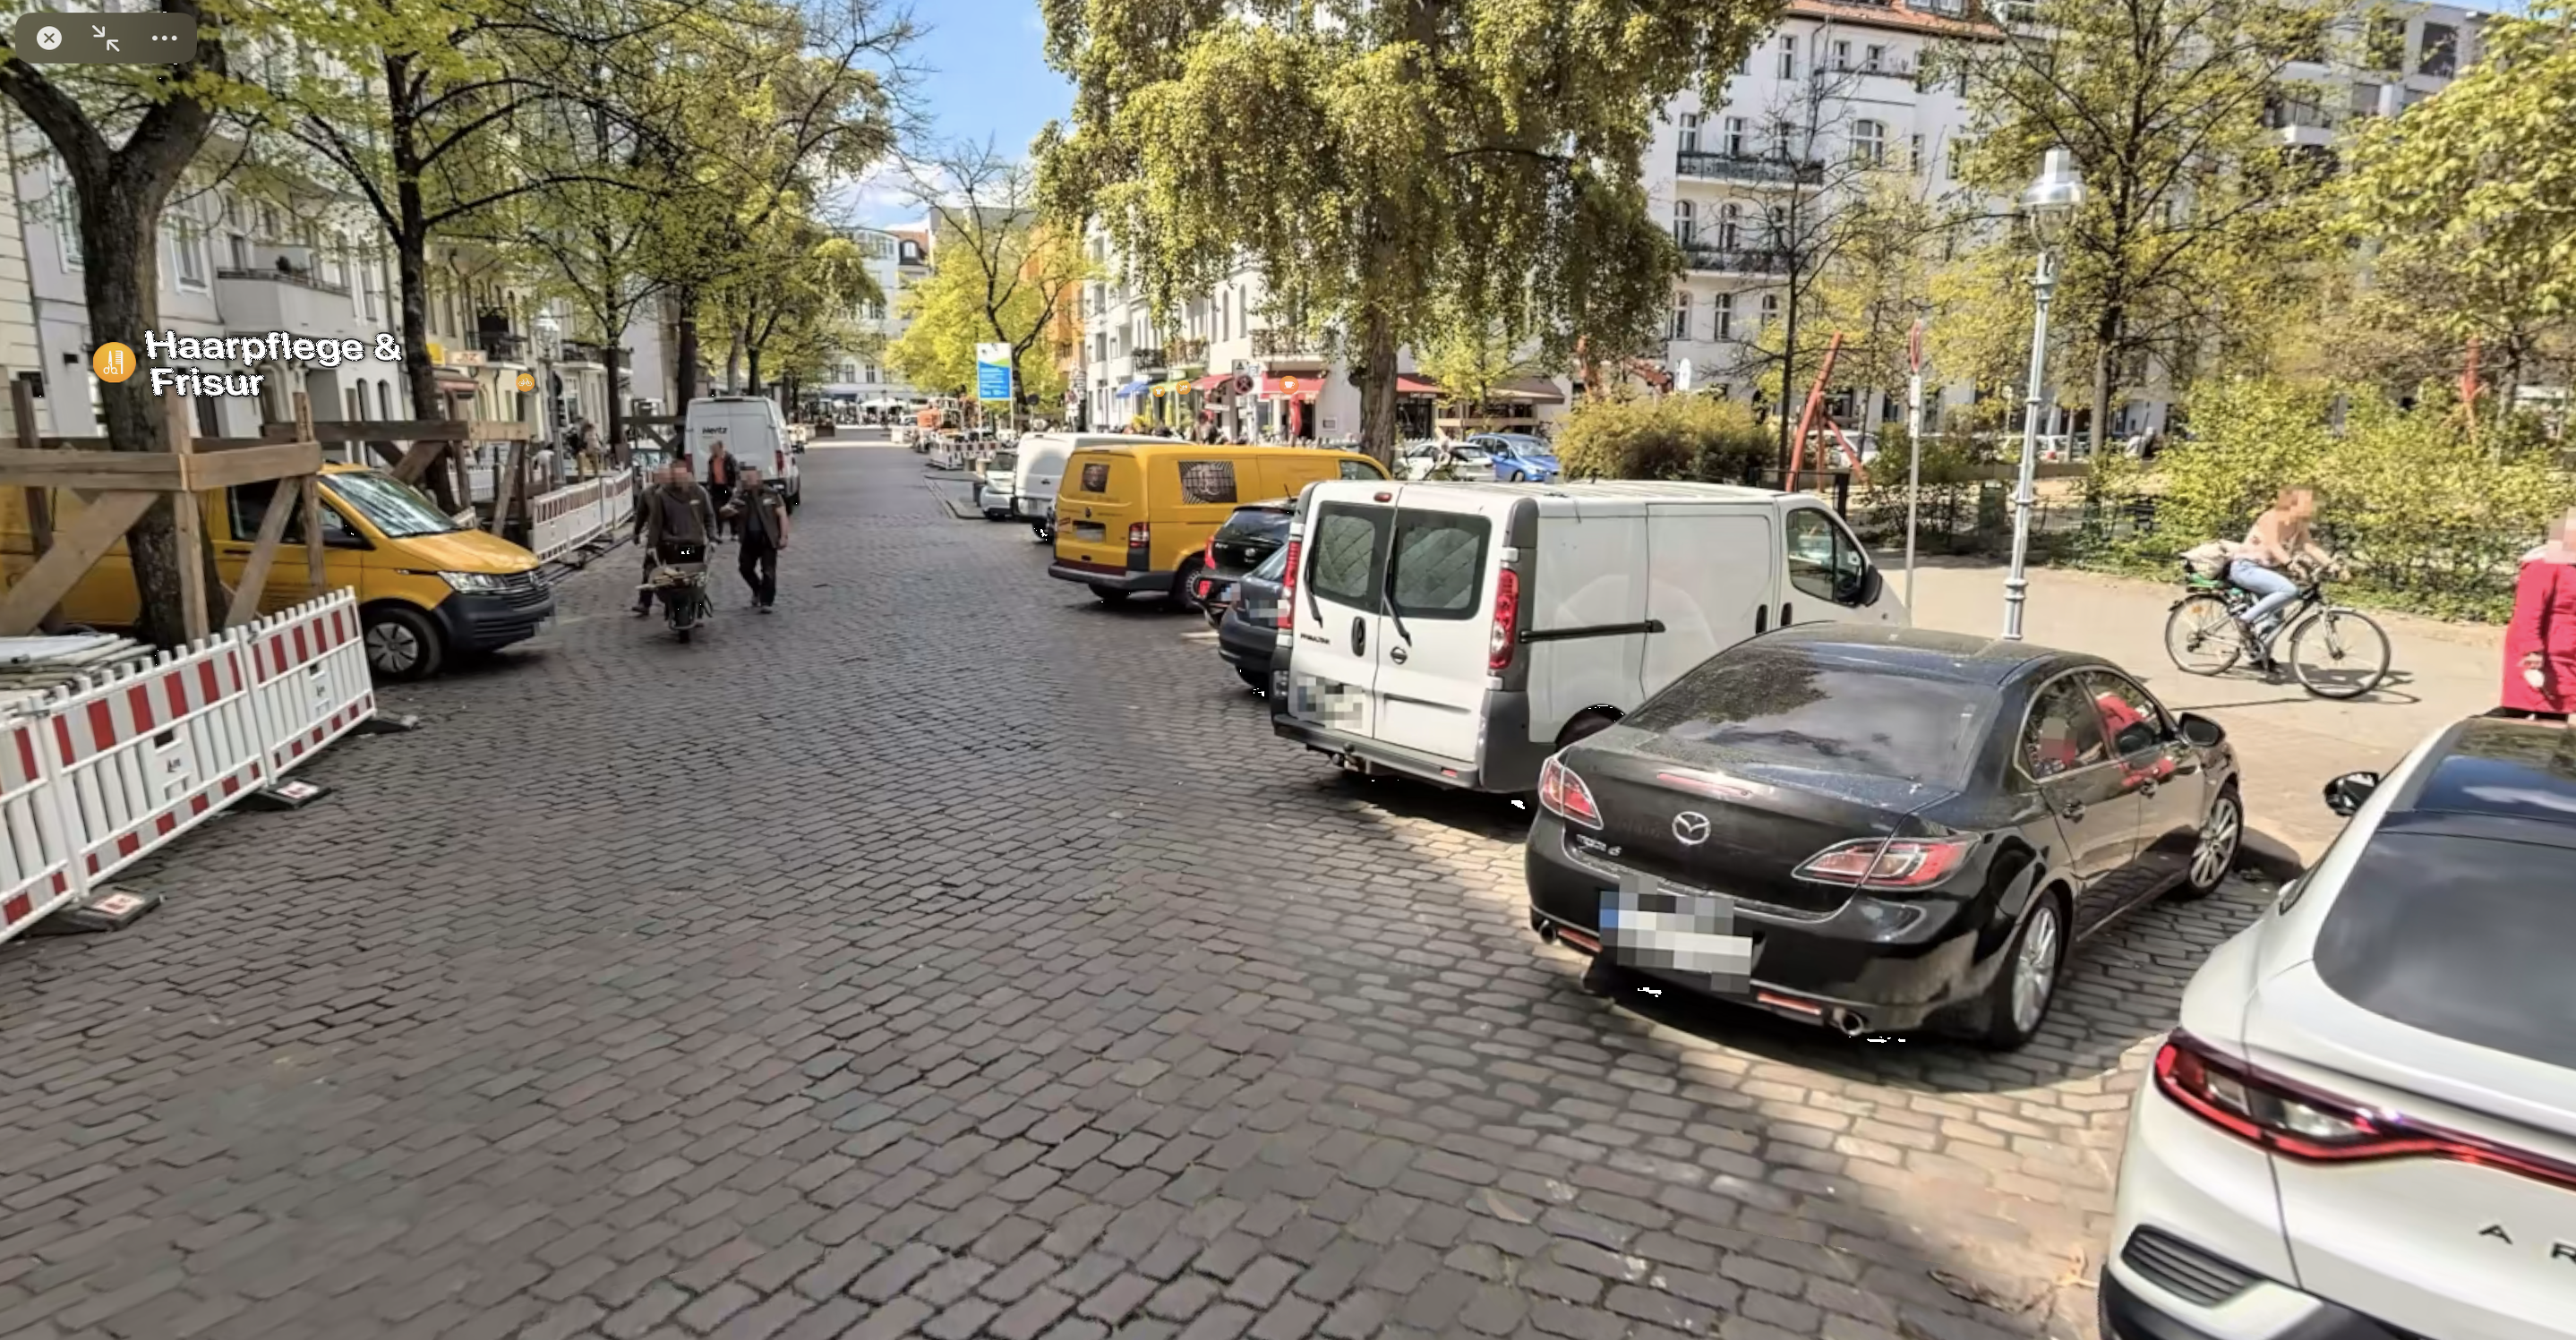
\includegraphics[width=\columnwidth]{fig/goethestr22.png}}
    \caption{%
        Straßburger Straße and Goethestraße in Berlin are paved with large cobblestones and the roads are contested by cars that are parking or searching for a parking spot. In contrast, the sidewalks are paved with flat-surfaced paving stones and are quiet due to the absence of shops, restaurants or cafes. (Source: Apple Maps)
    }%
    \label{fig:sidewalk}
    \vspace{-.5em}
\end{figure*}

\Cref{fig:sidewalk} also shows very likely reasons why these sections have very smooth bicycle rides.
The infrastructural conditions incentivize cyclists to prefer the sidewalks over the actual streets.
First, the cobblestones on the streets make it very unpleasant for cyclists to cycle on them.
Second, the sidewalks are wide, quiet, and paved with large flat-surfaced paving stones.
Third, the streets are contested by parking cars, or by cars searching for a parking spot, service vehicles, construction vehicles, etc. which will often block cyclists and also create safety hazards.
Considering these circumstances, it is not surprising to see good surface quality values in these two and other similar streets as cyclists are likely to (illegaly) use the sidewalks instead.
In fact, photos on Apple Maps (not included in this paper) actually show cyclists using the sidewalk instead.

\begin{table}%
\centering
\caption{Surface Quality Analysis Evaluation Results Showing Mean, Median and Standard Deviation of Sections With (Seemingly) Confusing Results}%
\label{tab:mismatch}
\resizebox{\columnwidth}{!}{
\begin{tabular}{cccccc}%
\toprule%
Street Name        & Surface     & GPS Location        & Mean & Median & Std. Dev.\\%
\midrule%
\midrule%
Straßburger Straße & Cobblestone & 52.532273,13.416521 & 1.43 & 1      & 0.87\\%
Goethestraße       & Cobblestone & 52.508889,13.308333 & 1    & 1      & 0\\%
\bottomrule&%
\end{tabular}%
}
\end{table}

\subsection{Related Work of CycleQuality}
\label{subsec:related_work_cyclequality}
Surface quality is usually quantified based on the International Roughness Index (IRI), e.g.,~\cite{sayers1986The}.
Traditionally, this was done using so-called profilographs (approximately resembling a large ladder with wheels) which are towed by a car or pushed manually.
A study from the 1980s~\cite{cumbaa1986road} found that they often break down and are difficult to maneuver in narrow streets which renders them infeasible for measuring the quality of bike lanes.
Furthermore, such measurement are very personnel-intensive which makes it unrealistic to apply them on a broad scale.

Taniguchi et al.~\cite{taniguchi2015evaluation} detect road hazards such as debris, potholes, or bumps.
For this, they attach an ultrasonic distance sensor to a bike handlebar, scanning the ground in front of the bicycle.
While the approach can warn cyclists about incoming bumps on the road ahead in real-time, this approach does not scale for city-wide analysis due to the sheer number of sensors needed.

Peng et al.~\cite{peng2019road} follow the same goal, using motion sensors instead of distance measurements.
Data is analyzed offline using a classifier which can identify asphalt, pebbles, and very bumpy underground.
In contrast to our work, their emphasis is on identifying specific surface \textit{types} rather than the surface \textit{quality}.
Also, their approach again requires dedicated hardware.

Zhou et al.~\cite{zhou2022smartphone} try to detect manhole covers.
For this, they analyze a video stream from a bike handlebar-mounted smartphone camera using a convolutional neural network.
While their approach is similar to ours regarding hardware, constantly recording video means high power consumption.
Furthermore, the phone needs to be mounted in an awkward angle which makes it impractical for every day use.

Luedemann et al.~\cite{luedemann2022bikevibes} use a smartphone app to record accelerometer data as an indicator for surface quality.
Their approach, however, relies on single rides and has no concept of aggregating data from multiple rides.

Similar to us, Yamaguchi et al.~\cite{yamaguchi2015simple} want to measure the surface quality.
To achieve highly precise results, they combine the smartphone motion sensors with a cyclometer.
This approach will always give more precise results than our approach but again requires dedicated hardware which renders a city-wide usage infeasible.

Beyond these, there are several car-centric approaches which either use dedicated hardware, e.g.,~\cite{paper_chen_crsm}, have very specific phone placement requirements, e.g.,~\cite{paper_daraghmi_surface_crowdsourcing}, or focus on detecting the transients, i.e., individual pot holes, e.g.,~\cite{paper_alam_surface_transients,paper_li_surface_transients,paper_lima_surface_transients}.


\subsection{Discussion of CycleQuality}
\label{subsec:discussion_cyclequality}
Overall, the results presented in this paper show, that our approach can derive surface quality information using data recorded in the SimRa app.
Nevertheless, it still has a number of limitations which we discuss in this section.

\subsubsection{Methodological Challenges}
\label{subsubsec:methodological_challenges_cyclequality}
Since the SimRa dataset consists of crowdsourced data generated by smartphones, the recorded data is very heterogeneous.
This comes from the fact that different smartphone models have different GPS modules and motions sensors, which leads to the problem that a road can be very smooth according to one smartphone and very rough according to another.
This problem is further aggravated by the wide range of different bicycle types, e.g., racing bicycles or mountain bikes, which in turn also heavily influence the vibrations the smartphone can sense.
To solve these problems, we rely on the \textit{law of large numbers} and compare how a section's surface quality was relative to the ride. 

\subsubsection{Preprocessing in SimRa}
\label{subsubsec:preprocessing_in_simra}
As input for our surface quality analysis pipeline, we used the SimRa dataset, since it is to our knowledge the only public dataset containing a very high number of anonymized individual rides in a non-aggregated form.
However, it is important to note, that SimRa was developed for identifying near miss incident hotspots in bicycle traffic.
For that, a relatively low accelerometer sampling rate of 50 Hz is used before further reducing the level of detail by calculating the moving average with a window size of 30 and then taking every fifth value.
While with this, it is possible to automatically detect near-miss incidents~\cite{karakaya2022cyclesense}, a higher resolution of data points would allow us to develop a more sophisticated measurement approach.
This would, however, further increase the disk space, memory, battery and bandwidth usage of the SimRa app and as we have shown in \cref{sec:eval}, the surface quality we derive are sufficiently precise for our intended use cases.

\subsubsection{Behavior of Cyclists}
\label{subsubsec:behavior_of_cyclists}
Due to the GPS inaccuracy, it is impossible to identify whether a cyclist used the actual road or the sidewalk.
For instance, as discussed in the previous section, \cref{fig:sidewalk} showing \textit{Straßburger Straße} in Berlin, would be expected to have poor results but in fact has surprisingly good values.
We believe that this is due to cyclists illegaly using the smooth sidewalk instead of the bumpy road.

Furthermore, cyclists will in practice also avoid the worst potholes and similar bumps if possible, i.e., these will usually be missing from our analysis.

\subsubsection{Sensor Inaccuracy}
\label{subsubsec:sensor_inaccuracy}
The inaccuracy of the GPS sensors~\cite{merry2019smartphone} combined with noise produced by the motion sensors of the smartphones form another limitation of the dataset.
We tried to partially address these limitations with our preprocessing steps but they can, of course, not be fully mitigated.
The only alternative would be using dedicated hardware which, however, will result in significantly less recorded rides due to the adoption barrier.

\subsubsection{Temporal Influences}
\label{subsubsec:temporal_influences}
The rides in the SimRa dataset date back up to 2019 and it is possible that the surface quality changed throughout the time.
One reason for that could be that the surface type is changed for example from cobblestones to asphalt or potholes and cracks are repaired.
This would presumably lead to better results after the change, but show up as two-peak distribution in our dataset.
When using this approach in practice, we hence propose to only consider the most recent rides.

Another temporal influence might be the weather.
On rainy, windy or snowy days, the surface quality of the road, especially with wet gravel, can suffer significantly, which is not considered by our surface quality analysis approach.
However, adding this factor to the analysis, would in our dataset reduce the validity of the results, since it would reduce the number of considered rides.


\subsection{Summary of CycleQuality}
\label{subsec:summary_cyclequality}
Cities all over the world aim to increase the modal share of bicycle traffic, e.g., to address emission problems, frequent traffic jams, but also to improve the citizens' health through more daily activity.
Aside from safety, a key influence factor for this is comfort, particularly in the form of the surface quality of cycling infrastructure.
Monitoring the surface quality manually, however, is infeasible due to the dimensions of such infrastructure.

In this paper, we proposed a crowdsensing approach in which cyclists record their daily rides using a smartphone app and the phone's built-in motion sensors.
We proposed a data processing pipeline that starts on the edge (i.e., the phone) and ends in a cloud backend.
Furthermore, we showed that our crowdsensing approach can indeed derive surface quality and implemented two use cases for using such data.



\section{Cyclist Model for SUMO}
\label{sec:sumo}
%Motivation
Active transportation modes such as cycling provide health benefits, alleviate traffic congestion, and reduce air pollution~\cite{goetschi2016cycling}.
In practice, however, cyclists often face a car-centric traffic infrastructure which has a significant impact on their (perceived) safety and also affects the attractiveness of cycling routes~\cite{karakaya2020simra, pedroso2016bicycle,aldred2018predictors}.
Changing this infrastructure to better accommodate cyclists and pedestrians requires significant planning efforts of city planners and traffic engineers.
Similarly, road traffic safety systems for vulnerable road users are often assessed using simulation.
Particularly the interaction with cars is relevant when it comes to V2X-based safety systems for cyclists~\cite{oczko2020integrating}.
Many of these studies rely on the open source simulation platform SUMO\footnote{https://www.eclipse.org/sumo/} (Simulation of Urban Mobility), which allows them to study the effects of infrastructure changes before implementing them on the streets.

In SUMO, vehicles and their dynamics are simulated individually~\cite{lopez2018microscopic}.
Unfortunately, the cyclist model is not particularly realistic -- cyclists can either be modeled to behave as slow cars or as fast pedestrians.
Several studies have already improved the bicycle model of SUMO.
For instance, Kaths et al.~\cite{kaths2016integration} investigated the intersection behavior of cyclists using camera traces and transferred findings into SUMO.
Also, Grigoropoulos et al.~\cite{grigoropoulos2019modelling} improved modeling of bicycle infrastructure at intersections while Heinovski et al.~\cite{heinovski2019modeling} created a virtual cycling environment to import real bicycle behavior directly into SUMO.
Nevertheless, the current cyclist behavior in SUMO is still rather unrealistic; so far, researchers have devoted much more effort to car models, e.g., \cite{chandler1958traffic,gazis1961nonlinear,gipps1981behavioural, leutzbach1986development,bando1995dynamical,krauss1998microscopic,treiber2000congested,salles2020extending}.
One reason for this is that, until recently, not enough data on real-world cyclist behavior have been available.
Today, crowdsourced data collection approaches such as SimRa\footnote{https://github.com/simra-project/}~\cite{karakaya2020simra} have made thousands of cycle tracks available as open data.

In this paper, we analyze the SimRa dataset regarding acceleration, deceleration, and velocity of cyclists as well as their left-turn behavior in four-way intersections.
We then use our findings to improve the cyclist model in SUMO.
Additionally, we add three more detailed cylist models for slow, medium and fast cyclists.
In this regard, we make the following contributions:
\begin{itemize}
    \item We show that SUMO's default bicycle simulation is not realistic,
    \item we improve bicycle simulation of SUMO by deriving new parameters for that vehicle type in SUMO,
    \item we add three new bicycle simulation models - slow, mediumd and fast - to SUMO by splitting the SimRa dataset into slow, medium and fast rides.
    \item we develop an intersection model which captures cyclists' left-turn behavior at intersections in a more realistic way, and
    \item we compare our improvements to SUMO's default bicycle simulation, using the SimRa dataset as a ground truth.
\end{itemize}

This paper is an extension of our previous work~\cite{karakaya2022realistic}.
The main new contributions are:
\begin{itemize}
\item We rerun all analyses of the original paper using significantly more rides which have become available in the time period since starting our original paper.
\item We complement the general cyclist model from our original paper with three dedicated models covering the behavior of cyclist groups clustered by their average velocity.
    For each of the three models, we also derive distributions of left-turn, acceleration, and maximum velocity behavior.
\item For both the general and the three dedicated cyclist models, we also derive deceleration behavior as a distribution.
\item We implement all new contributions as SUMO plugins and have successfully reimplemented the cyclist model from our original paper in SUMO core.
    We are currently in the process of finalizing an implementation of the extensions of this paper also in SUMO core.
\item We evaluate all four cyclist models against the default cyclist model of SUMO using scenarios from Berlin, Munich, and Hanover, Germany
\end{itemize}


\subsection{Cycling Behavior in SimRa and SUMO}
\label{subsec:cycling_behavior_in_simra_and_sumo}


\subsubsection{Preprocessing}
\label{subsubsec:preprocessing_sumo}

\subsubsection{Categorizing by Velocity}
\label{subsubsec:categorizing_by_velocity_preprocessing}

\subsubsection{Acceleration}
\label{subsubsec:acceleration_preprocessing}

\subsubsection{Deceleration}
\label{subsubsec:deceleration_preprocessing}

\subsubsection{Velocity}
\label{subsubsec:velocity_preprocessing}

\subsubsection{Left-turn Behavior at Intersections}
\label{subsubsec:left-turn_behavior_at_intersections_preprocessing}


\subsection{Improving SUMO's Bicycle Simulation}
\label{subsec:improving_sumos_bicycle_simulation}


\subsubsection{Longitudinal Kinematic Behavior}
\label{subsubsec:longitudinal_kinematic_behavior}

\subsubsection{Left-turn Behavior at Intersections}
\label{subsubsec:left-turn_behavior_at_intersections}

\subsubsection{Different Cyclist Models}
\label{subsubsec:different_cyclist_models}


\subsection{Evaluation of the Cyclist Model for SUMO}
\label{subsec:evaluation_sumo}


\subsubsection{Simulation Setup}
\label{subsubsec:simulation_setup}

\subsubsection{Acceleration}
\label{subsubsec:acceleration_evaluation}

\subsubsection{Deceleration}
\label{subsubsec:deceleration_evaluation}

\subsubsection{Velocity}
\label{subsubsec:velocity_evaluation}

\subsubsection{Left-turn Behavior at Intersections}
\label{subsubsec:left-turn_behavior_at_intersections_evaluation}

\subsubsection{Combining Intersection Model and Kinematic Extension}
\label{subsubsec:combinin_intersection_model_and_kinematic_extension}


\subsection{Discussion of the Cyclist Model for SUMO}
\label{subsec:discussion_sumo}


\subsubsection{Methodological Challenges}
\label{subsubsec:methodological_challenges_sumo}

\subsubsection{Dataset Choice as Ground Truth}
\label{subsubsec:dataset_choice_as_ground_truth}

\subsubsection{Limitations}
\label{subsubsec:limitations_sumo}

\subsubsection{E-bikes}
\label{subsubsec:e-bikes}

\subsection{Summary of Bicycle Simulation for SUMO}
\label{subsec:summary_sumo}